The Engine for Likelihood-Free Inference (ELFI) \cite{1708.00707}
is a Python package dedicated to Likelihood-Free Inference (LFI). ELFI
models in a convenient manner all the fundamental components of a
probabilistic model such as priors, simulators, summaries and
distances. Furthermore, ELFI already supports some recently proposed
likelihood-free inference methods.

\subsubsection{Modelling}
\label{sec:modelling}

ELFI models the probabilistic model as a Directed Acyclic Graph (DAG);
it implements this functionality based on the package
\pinline{NetworkX}, which is designed for creating general purpose
graphs. Although not restricted to that, in most cases the structure
of a likelihood-free model follows the pattern presented in
figure~\ref{fig:elfi}; there are edges that connect the prior
distributions to the simulator, the simulator is connected to the
summary statistics that consequently are connected to the
distance. The distance is the output node. Samples can be obtained
from all nodes through sequential sampling. The nodes that are defined
as \pinline{elfi.Prior}\footnote{The \pinline{elfi.Prior} functionality
  is a wrapper around the \pinline{scipy.stats} package.} are automatically
considered as the parameters of interest and are the only nodes that,
apart from sampling, should also provide PDF evaluation. The function
passed as argument in the \pinline{elfi.Summary} node can be any valid
Python function. Finally, the observations should be passed in the
appropriate node through the argument \pinline{observed}.

\begin{figure}[!ht]
    \begin{center}
      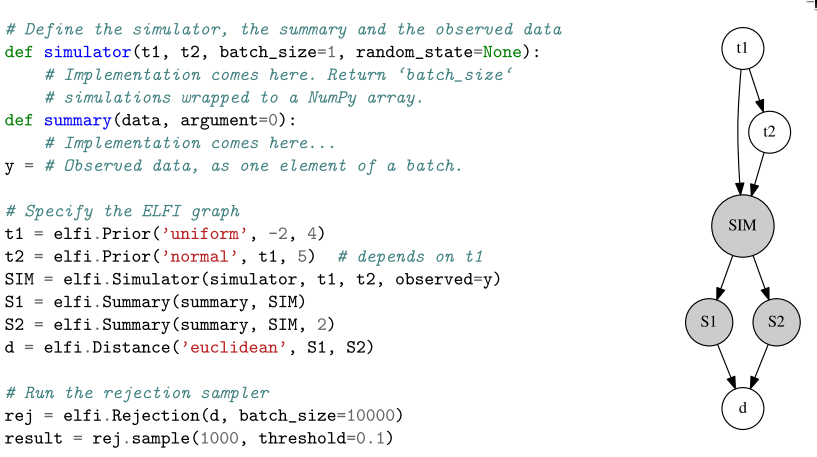
\includegraphics[width=0.8\textwidth]{./latex_files/images/chapter2/elfi.png}
    \end{center}
    \caption[Baseline example for creating an \pinline{ELFI} model]{Baseline example for creating an \pinline{ELFI} model. Image taken from \cite{1708.00707}}
    \label{fig:elfi}
\end{figure}


\subsubsection{Inference Methods}
\label{sec:inference-methods}

The inference Methods implemented at the ELFI follow some common
guidelines;

\begin{itemize}
\item the initial argument should is the output node of the model. It
  is followed by the rest hyper-parameters of the method.
\item each inference method provides a central sampling
  functionality. In most cases it is named
  \pinline{<method_name>.sample()}.
\end{itemize}

The collection of likelihood-free inference methods implemented so far
contain the \textit{ABC Rejection Sampler}, the \textit{Sequential
  Monte Carlo ABC Sampler} and the \textit{Bayesian Optimisation for
  Likelihood-Free Inference (BOLFI)}. The latter has methodological
similarities to the ROMC method that we implement in the current work.
